\section{Bloco de Alumínio}
\label{aluminio_01}


\begin{table}[ht!]

	\begin{tabular}{r l|l p{12cm} }
		
		\textcolor{gray}{Especificação} &&& 	{Bloco de Alumínio}\\
		\textcolor{gray}{Data} &&& 				{09/02/2015}\\
        \textcolor{gray}{Beneficiado} &&&		{Metal Center Aços e Metais LTDA}\\
        \textcolor{gray}{CNPJ} &&& 				{40.253.676/0001-01}\\
        \textcolor{gray}{Número Nota} &&& 		{10434}\\
		\textcolor{gray}{Quantidade} &&& 		{1}\\
		\textcolor{gray}{Valor} &&& 			{R\$1.790,00}\\
		\textcolor{gray}{Data Sheet} &&& 		{-}\\

		\textcolor{gray}{Função no projeto} &&& {Bloco de alumínio a ser
		usinado e ser utilizado como case da eletrônica embarcada.}\\
		\textcolor{gray}{Razão da Escolha} &&& {Pronta entrega.}

	\end{tabular}
\end{table}

\newpage
\subsection{Foto do Material}
\begin{figure}[H]
 \centering
 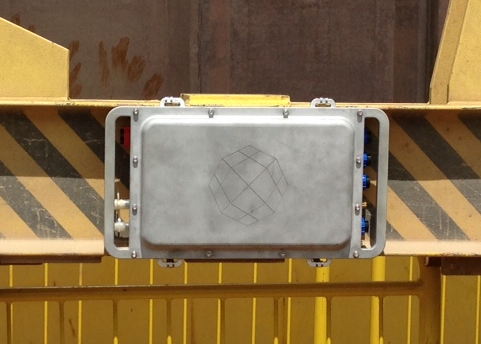
\includegraphics[width=1\columnwidth]{Aluminio/foto.png}
 \caption{Case da eletrônica embarcada}
\end{figure}

\subsection{Nota Fiscal}
\begin{figure}[H]
 \centering
 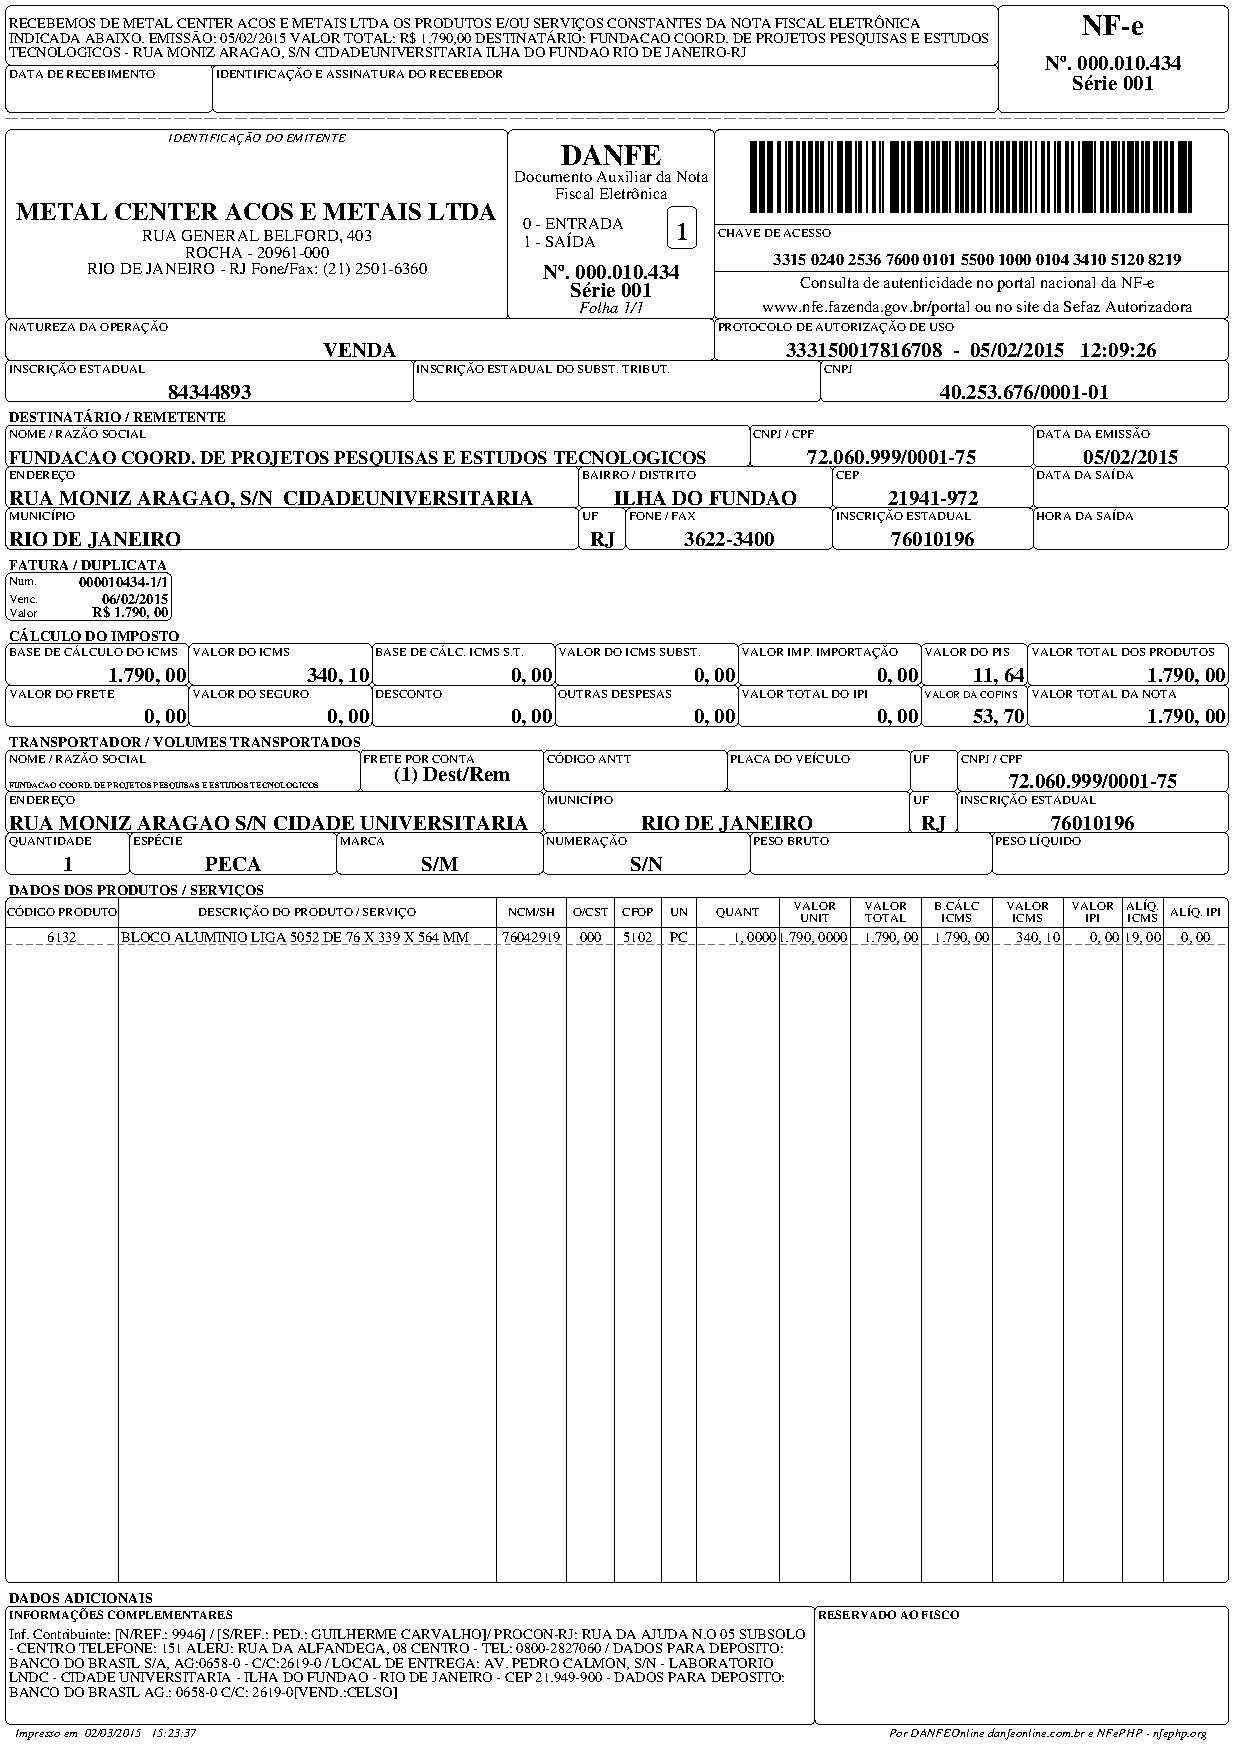
\includegraphics[width=0.9\columnwidth]{Aluminio/nota.pdf}
 \caption{Nota fiscal do Bloco de Alumínio}
 \end{figure}